\chapter{Demo Facility}\label{cha:demoFacility}
Physical creation of the demo facility that showcases the possibilities of the chosen wearable in the process of order picking in a warehouse. As the demo facility is not yet existing the implementation cannot be discussed and explained here, this chapter will therefore focus on the planned infrastructure, the existing design and what is planned for the demo facility in the future. 

There is also a major difference between the demo facility task that will be explained in this report and the task given in the logwear website. \citep{website:logwear} The task that will be executed here will be creating a demo facility in a physical \gls{sandbox} environment and the task explained in the work package on the logwear homepage is about implementing the improved process, using a wearable, at a pilot company and observing the results.

\section{Infrastructure}
The infrastructure of the demo facility is divided into two areas, the first area is the 
\begin{description}
	\item[Mock WMS] \hfill \\
		A mock \gls{wms} that allows to store different orders and edit them to have a more realistic demo. While not all functionality has to given, the data has to be persistent and easily resettable to allow showcasing a demo case multiple times. The mock \gls{wms} is living on an azure server and is a \gls{mssql} database.
	\item[Rest API] \hfill \\
		A \gls{rest} \gls{api} that is used to connect to the mock \gls{wms} from an outside perspective, in this case from the communication layer, see subsection \ref{subsec:communication}.
	\item[Communication Layer] \hfill \\
		The communication layer will be living on a server with a connection to the \gls{db} \gls{api} and a connection to the wearable.
	\item[Wearable] \hfill \\
		The wearable will need to connect to the communication layer and process input and output.
\end{description}

The mock \gls{wms} and the \gls{rest} \gls{api} are insignificant parts of the implementation, therefore not a lot of thought was put into the decision on choosing these technologies was done out of curiosity for these technologies or being the most comfortable with them respectively.

\section{Demo Scenario}
The demo scenario explains the process that will be executed during the demo facility. Therefore describing the actions taken in detail, but ignoring how they will be executed, e.g. with or without a wearable. 

\begin{figure}[htbp]
	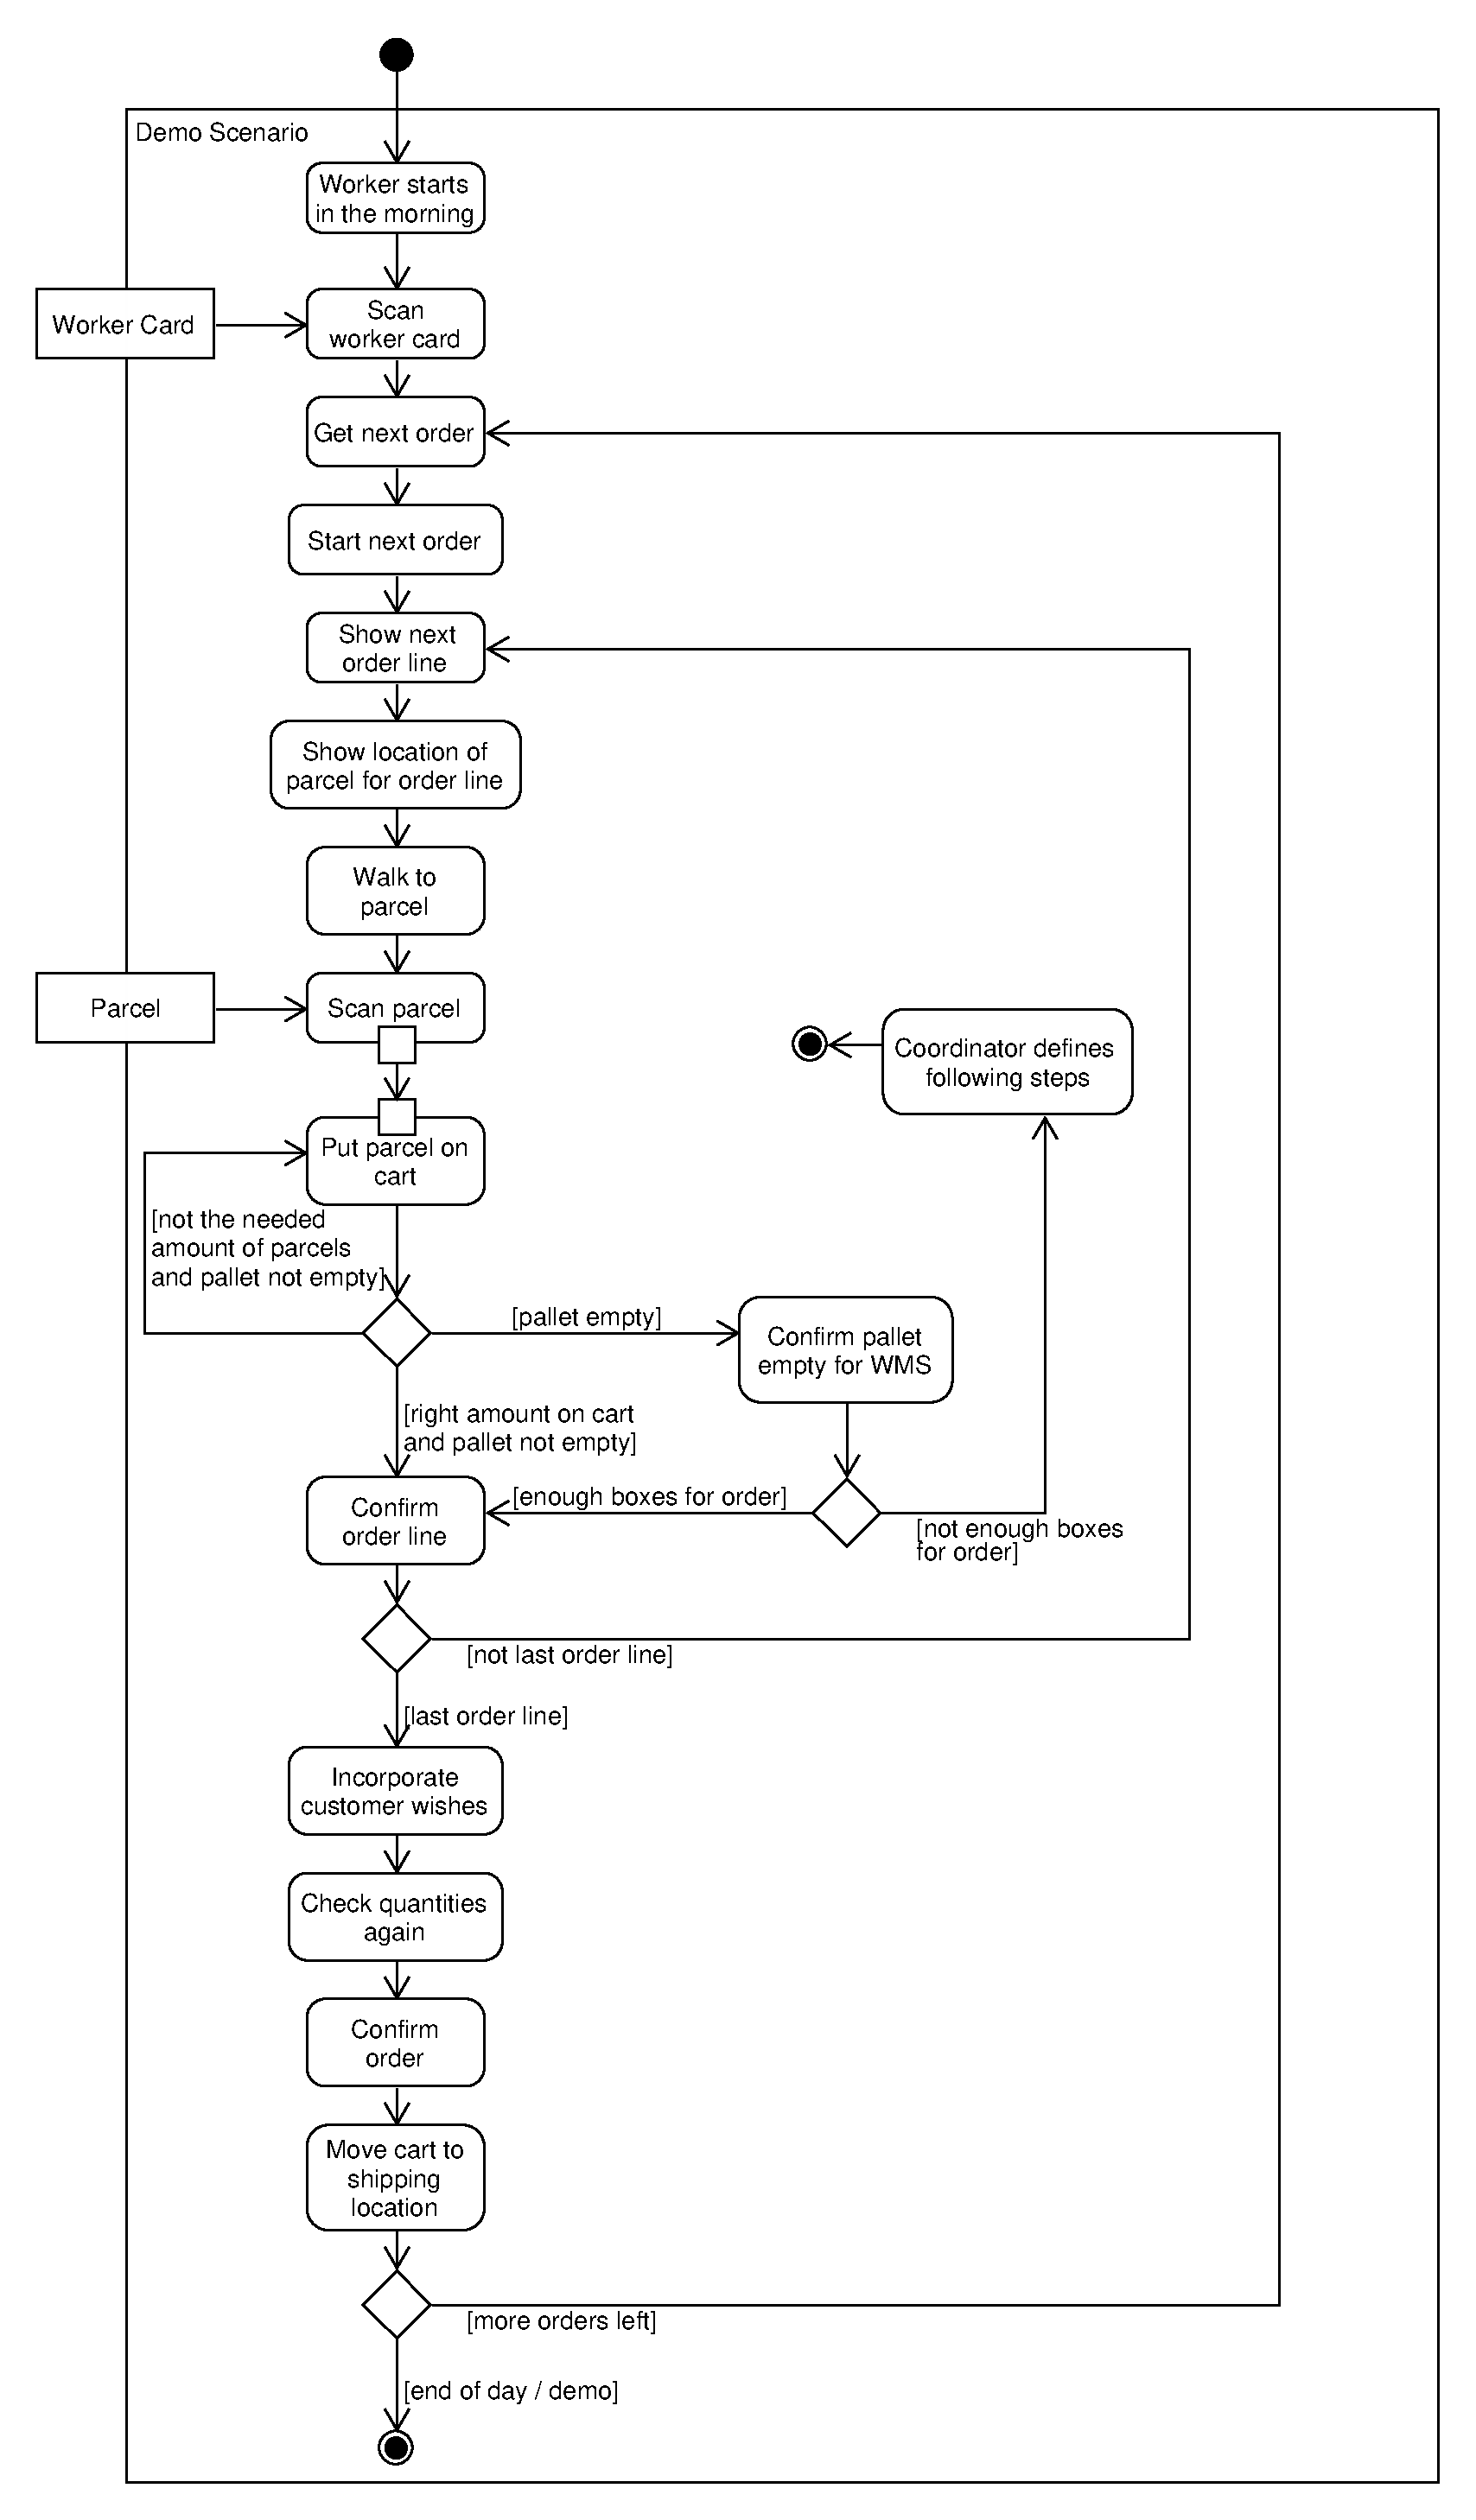
\includegraphics[height=\textheight]{images/activityDiagram_demoScenarioNoExceptions}
	\caption{Activity Diagram Demo Scenario}
	\label{fig:activityDemoScenario}
\end{figure}



\section{Design}
The general design for the demo facility application will be based on the reference model described in chapter \ref{cha:reference}. 
\section{Planning}
In the future for this task, there will be multiple wearables tried out and then decided which wearable will be used for the demo facility, as described in section \ref{sec:wearables}. Afterwards an application will be written for that wearable, to improve the process chosen in \ref{sec:processes}. 

This application will at least include the functionalities to:
\begin{itemize}
	\item Divide a given room in multiple sectors, to address a single part of the room with a given location string.
	\item Reset the case to allow multiple showcases of the demo.
	\item Allow scanning of \gls{id}s on \gls{parcel}s and pallets.
	\item Send confirmations to the \gls{wms}, that an action has been completed.
\end{itemize}

For the demo environment, an area will be rented that allows to place a rack in there with \gls{parcel}s. The \gls{parcel}s will be equipped with an \gls{id} that can be scanned with the chosen wearable.

When the implementation of the demo application is finished a second one could be started to show \gls{sme} the differences between the possibilities different wearables give the user.